% =====================================================================
%  TP5 - Simulacion de Sistemas - Grupo 5 (Comision \comision, ver mas abajo)
%  Presentacion oral (13 min): evacuacion de una sala, esquema hibrido EDMD + TSDMD
%
%  Formato segun docs/GuiaPresentaciones.md (misma plantilla que TP2, TP3 y TP4):
%   - 1.2  diapositivas numeradas
%   - 1.6  poco texto, sin parrafos
%   - 1.7  las figuras NO llevan titulo ni caption; los parametros de la
%          corrida van AL COSTADO de la figura (macro \params)
%   - 1.9  notacion cientifica con potencias de 10 (supraindice), punto decimal
%   - 1.12 outertheme miniframes
%   - 1.13 secciones separadas por una diapositiva con solo el titulo
%
%  Cada diapositiva lleva, justo antes de \begin{frame}, un marcador
%      % SLIDE <id> | V:<A|B|C> | T:<segundos>
%  (V = voz que presenta, T = segundos planeados).
%
%  Insumos GENERADOS (no se editan a mano):
%      figuras/*.png   py/python3 TP5/presentacion/make_pres_figures.py
%      tablas.tex      python3 TP5/presentacion/pres_format.py
%      links.tex       python3 TP5/presentacion/links.py --emit-tex
%      frame_t.tex     build_deck.py (instante comun de los fotogramas, de MANIFEST.json)
%
%  El cuerpo vive en secciones/*.tex (una por seccion de la Guia); compilar con
%  build_deck.py, que corre el lint antes de pdflatex.
%
%  Compilar (MiKTeX en Windows; el TeX Live de WSL no tiene babel-spanish):
%      cd TP5/presentacion && pdflatex -interaction=nonstopmode -halt-on-error presentacion.tex
%  (dos pasadas: la segunda resuelve el indice de los miniframes)
% =====================================================================
\pdfsuppressptexinfo=-1 % el PDF no guarda rutas ni version del compilador (T-10-06)
\documentclass[aspectratio=169]{beamer}

\usetheme{Boadilla}
\useoutertheme{miniframes}
\usecolortheme{whale}

\usepackage[utf8]{inputenc}
\usepackage[T1]{fontenc}
\usepackage[spanish,es-noquoting]{babel}
\usepackage{amsmath,amssymb,graphicx,booktabs,url}
% Punto decimal tambien en modo matematico (D-09): babel-spanish usa coma por defecto.
\decimalpoint
\usepackage{tikz}
\usetikzlibrary{arrows.meta,shapes.multipart,positioning,fit,backgrounds,calc,decorations.pathreplacing}

% Comision: unico lugar donde aparece en el texto (D-03). Valores: S o S2.
\newcommand{\comision}{S}

\graphicspath{{figuras/}{./}}
% Generado por presentacion/links.py --emit-tex a partir de links.json. No editar.
% Uso: \videolink{<id>} (requiere el paquete url).
\expandafter\def\csname linkurl@tsdmd_n500\endcsname{\textbf{\textcolor{red}{PENDIENTE subir video tsdmd\_n500}}}
\expandafter\def\csname linkurl@edmd_n500\endcsname{\textbf{\textcolor{red}{PENDIENTE subir video edmd\_n500}}}
\expandafter\def\csname linkurl@hybrid_n500\endcsname{\textbf{\textcolor{red}{PENDIENTE subir video hybrid\_n500}}}

% Generado por TP5/presentacion/pres_format.py desde TP5/data/studies/figures. No editar.
\newcommand{\tablaTevac}{%
\begin{tabular}{lrrrr}
\toprule
Esquema & Completas (tasa) & $t_{\mathrm{evac}}$ (s) & Razón & $z$ \\
\midrule
TSDMD & $15/32 = 0.47$ & $(9.69 \pm 0.14)\times 10^{2}$ & -- & -- \\
EDMD & $12/24 = 0.50$ & $(2.12 \pm 0.09)\times 10^{2}$ & $0.22$ & $-44.3$ \\
Híbrido & $11/24 = 0.46$ & $(9.6 \pm 0.2)\times 10^{2}$ & $0.99$ & $-0.4$ \\
\bottomrule
\end{tabular}}
\newcommand{\tablaWall}{%
\begin{tabular}{lrrr}
\toprule
Esquema & Completas & Ejecución (s) & Razón \\
\midrule
TSDMD & 10/10 & $(1.57 \pm 0.03)\times 10^{2}$ & -- \\
EDMD & 10/10 & $(3.05 \pm 0.14)\times 10^{2}$ & $1.9$ \\
Híbrido & 10/10 & $(2.11 \pm 0.03)\times 10^{2}$ & $1.3$ \\
\bottomrule
\end{tabular}}
\newcommand{\tablaSweep}{%
\begin{tabular}{lrrr}
\toprule
Híbrido & Completas & Ejecución (s) & $t_{\mathrm{evac}}$ (s) \\
\midrule
$T = 0$ s & 5/5 & $67 \pm 8$ & $(1.13 \pm 0.07)\times 10^{2}$ \\
$T = 0.1$ s & 2/5 & $26.6 \pm 0.3$ & $(3.43 \pm 0.02)\times 10^{2}$ \\
$T = 0.25$ s & 3/5 & $31.4 \pm 1.1$ & $(3.61 \pm 0.07)\times 10^{2}$ \\
$T = 0.5$ s & 1/5 & $36.4$ (n=1) & $3.36\times 10^{2}$ (n=1) \\
$T = 1$ s & 4/5 & $47.5 \pm 1.9$ & $(3.540 \pm 0.016)\times 10^{2}$ \\
$T = 2$ s & 4/5 & $68.6 \pm 1.2$ & $(3.3 \pm 0.2)\times 10^{2}$ \\
$T = 3$ s & 3/5 & $91 \pm 2$ & $(3.4 \pm 0.2)\times 10^{2}$ \\
\midrule
TSDMD puro & 4/5 & $22.2 \pm 1.4$ & $(3.62 \pm 0.12)\times 10^{2}$ \\
EDMD puro & 5/5 & $68 \pm 8$ & $(1.13 \pm 0.07)\times 10^{2}$ \\
\bottomrule
\end{tabular}}
\newcommand{\tablaPendientes}{%
\begin{tabular}{llr}
\toprule
Variante & Esquema & Pendiente \\
\midrule
a & TSDMD & $2.3$ \\
a & EDMD & $1.6$ \\
a & Híbrido & $1.9$ \\
b & TSDMD & $1.7$ \\
b & EDMD & $2.3$ \\
b & Híbrido & $1.8$ \\
\bottomrule
\end{tabular}}
\newcommand{\tablaExito}{%
\begin{tabular}{llrr}
\toprule
Estudio & Esquema & $N$ & Completas \\
\midrule
base, estadística & TSDMD & 500 & 15/32 \\
base, estadística & EDMD & 500 & 12/24 \\
base, estadística & Híbrido & 500 & 11/24 \\
base, tiempos & TSDMD & 500 & 10/10 \\
base, tiempos & EDMD & 500 & 10/10 \\
base, tiempos & Híbrido & 500 & 10/10 \\
escalado a & TSDMD & 100 & 3/3 \\
escalado a & TSDMD & 200 & 3/3 \\
escalado a & TSDMD & 400 & 3/3 \\
escalado a & TSDMD & 700 & 2/3 \\
escalado a & TSDMD & 1000 & 2/3 \\
escalado a & EDMD & 100 & 1/3 \\
escalado a & EDMD & 200 & 1/3 \\
escalado a & EDMD & 400 & 1/3 \\
escalado a & EDMD & 700 & 1/3 \\
escalado a & EDMD & 1000 & 2/3 \\
escalado a & Híbrido & 100 & 2/3 \\
escalado a & Híbrido & 200 & 1/3 \\
escalado a & Híbrido & 400 & 1/3 \\
escalado a & Híbrido & 700 & 2/3 \\
escalado a & Híbrido & 1000 & 2/3 \\
escalado b & TSDMD & 100 & 2/3 \\
escalado b & TSDMD & 200 & 0/3 \\
escalado b & TSDMD & 400 & 3/3 \\
escalado b & TSDMD & 700 & 1/3 \\
escalado b & TSDMD & 1000 & 1/3 \\
escalado b & EDMD & 100 & 3/3 \\
escalado b & EDMD & 200 & 2/3 \\
escalado b & EDMD & 400 & 1/3 \\
escalado b & EDMD & 700 & 1/3 \\
escalado b & EDMD & 1000 & 2/3 \\
escalado b & Híbrido & 100 & 3/3 \\
escalado b & Híbrido & 200 & 1/3 \\
escalado b & Híbrido & 400 & 3/3 \\
escalado b & Híbrido & 700 & 1/3 \\
escalado b & Híbrido & 1000 & 1/3 \\
barrido de $T$ & TSDMD & 200 & 4/5 \\
barrido de $T$ & EDMD & 200 & 5/5 \\
barrido de $T$ ($T = 0$) & Híbrido & 200 & 5/5 \\
barrido de $T$ ($T = 0.1$) & Híbrido & 200 & 2/5 \\
barrido de $T$ ($T = 0.25$) & Híbrido & 200 & 3/5 \\
barrido de $T$ ($T = 0.5$) & Híbrido & 200 & 1/5 \\
barrido de $T$ ($T = 1$) & Híbrido & 200 & 4/5 \\
barrido de $T$ ($T = 2$) & Híbrido & 200 & 4/5 \\
barrido de $T$ ($T = 3$) & Híbrido & 200 & 3/5 \\
\bottomrule
\end{tabular}}

% Generado por TP5/presentacion/make_explore_table.py. No editar.
\newcommand{\tablaExplora}{%
\begin{tabular}{lrrr}
\toprule
Variante & Completas & Ejecución (s) & $t_{\mathrm{evac}}$ (s) \\
\midrule
TSDMD & 4/6 & $24.7 \pm 1.7$ & $(3.43 \pm 0.17)\times 10^{2}$ \\
EDMD & 2/6 & $90 \pm 20$ & $(1.30 \pm 0.16)\times 10^{2}$ \\
Híbrido actual & 5/6 & $41.9 \pm 1.4$ & $(3.43 \pm 0.12)\times 10^{2}$ \\
Retorno cada $10$ pasos & 5/6 & $35.2 \pm 0.6$ & $(3.54 \pm 0.09)\times 10^{2}$ \\
Zona de $6\un{m}$ + retorno & 5/6 & $34.1 \pm 0.5$ & $(3.50 \pm 0.07)\times 10^{2}$ \\
\bottomrule
\end{tabular}}

% Generado por TP5/presentacion/make_extra_kappa0.py. No editar.
\newcommand{\tablaKappa}{%
\begin{tabular}{llrr}
\toprule
Esquema & $\kappa$ & Completas (tasa) & $t_{\mathrm{evac}}$ (s) \\
\midrule
TSDMD & $2.4\times 10^{5}$ & $15/32 = 0.47$ & $(9.69 \pm 0.14)\times 10^{2}$ \\
TSDMD & $0$ & $13/14 = 0.93$ & $(1.456 \pm 0.010)\times 10^{2}$ \\
Híbrido & $0$ & $13/14 = 0.93$ & $(1.456 \pm 0.009)\times 10^{2}$ \\
\bottomrule
\end{tabular}}

% Generado por build_deck.py desde figuras/MANIFEST.json. No editar.
\newcommand{\framet}{13.5}


% Unidades sin cursiva (Guia 1.9): $L = 50\un{m}$.
\newcommand{\un}[1]{\,\mathrm{#1}}

% Guia 3.5: vectores en negrita sin italica, escalares en italica sin negrita.
\newcommand{\vect}[1]{\mathbf{#1}}

\setbeamertemplate{navigation symbols}{}
\setbeamertemplate{footline}[frame number]

\AtBeginSection[]{%
  \begin{frame}[plain]
    \vfill
    \begin{beamercolorbox}[sep=8pt,center]{title}
      \usebeamerfont{title}\insertsection
    \end{beamercolorbox}
    \vfill
  \end{frame}
}

% Parametros de la corrida al costado de cada figura (Guia 1.7).
\newcommand{\params}[1]{{\footnotesize #1}}

% --- Modo de compilacion: entrega (default) vs. vivo -----------------
% `vivo` lo usa build_pptx.py: cada \animacion deja un rectangulo magenta del tamano
% exacto del fotograma, y el script pone el GIF encima en el .pptx.
\providecommand{\modo}{entrega}
\def\modovivo{vivo}
\definecolor{huecoanim}{RGB}{255,0,255}
\newcommand{\soloentrega}[1]{\ifx\modo\modovivo\else#1\fi}
% #1 id del video (links.json), #2 fotograma fijo (\includegraphics).
\newcommand{\animacion}[2]{%
  \ifx\modo\modovivo
    \sbox0{#2}\textcolor{huecoanim}{\rule{\wd0}{\ht0}}%
  \else
    #2%
  \fi}

% Link explicito al video (Guia 2.4.8): lo define links.tex desde links.json.
\newcommand{\videolink}[1]{{\scriptsize\color{blue}\csname linkurl@#1\endcsname}}

% Colores de los esquemas: los mismos que study_common.STUDY_COLORS.
\definecolor{tsdmdc}{HTML}{1F4E79}
\definecolor{edmdc}{HTML}{C0392B}
\definecolor{hybc}{HTML}{2E7D32}

\title[Evacuación híbrida]{Evacuación de una sala: esquema híbrido EDMD + TSDMD}
\author[Grupo 5]{Lucas Di Candia \and Juan Francisco Palermo \and Gonzalo Sharif Curi Martinez}
\institute[ITBA]{Grupo 5 --- Comisión \comision, Instituto Tecnológico de Buenos Aires}
\date{72.25 Simulación de Sistemas --- Trabajo Práctico N\textdegree{}5 --- 2026}

\hypersetup{pdftitle={TP5 - Evacuación de una sala: esquema híbrido EDMD + TSDMD},
            pdfauthor={Grupo 5}}

\begin{document}

% SLIDE title | V:A | T:12
\begin{frame}[plain]
  \titlepage
\end{frame}

% =====================================================================
\section{Introducción}
% =====================================================================
%  Introduccion (2 diapositivas, Guia 2.1: sin sistema ni metodo particular)
% =====================================================================

% SLIDE intro_real | V:A | T:25
\begin{frame}{Evacuación de una sala}
  \begin{columns}[c]
    \begin{column}{0.56\textwidth}
      \begin{itemize}
        \item Sala cuadrada con una única puerta estrecha.
        \item Lejos de la puerta: zona diluida, movimiento casi rectilíneo, contactos raros.
        \item En la puerta: cuello de botella, contactos continuos.
        \item Régimen mixto: contactos raros lejos de la puerta, continuos en la cola.
      \end{itemize}
    \end{column}
    \begin{column}{0.40\textwidth}
      \centering
      \begin{tikzpicture}[scale=0.95]
        \draw[thick,gray] (-1.9,-1.9) -- (-0.3,-1.9);
        \draw[thick,gray] (0.3,-1.9) -- (1.9,-1.9);
        \draw[thick,gray] (-1.9,-1.9) -- (-1.9,1.9) -- (1.9,1.9) -- (1.9,-1.9);
        \foreach \x/\y in {-1.4/1.4, -0.6/1.5, 0.3/1.3, 1.2/1.5, -1.5/0.5, -0.8/0.7,
                           0.7/0.6, 1.4/0.4, -1.2/-0.2, 0.2/-0.1, 1.0/-0.3}
          \fill[gray!60] (\x,\y) circle (0.11);
        \foreach \x/\y in {-0.35/-1.15, 0.0/-1.2, 0.35/-1.15, -0.55/-0.85, -0.2/-0.8,
                           0.2/-0.85, 0.55/-0.8, -0.35/-0.5, 0.0/-0.5, 0.35/-0.5}
          \fill[gray!90] (\x,\y) circle (0.11);
        \node[font=\scriptsize,gray!70!black] at (0,-2.25) {puerta};
        \node[font=\scriptsize,gray!70!black] at (-0.2,0.95) {diluida};
        \node[font=\scriptsize,gray!70!black] at (1.25,-1.15) {cola};
      \end{tikzpicture}
    \end{column}
  \end{columns}
\end{frame}

% SLIDE intro_sfm | V:A | T:40
\begin{frame}{Modelo de fuerza social, solo contacto}
  \small
  \[
    m\,\dot{\vect v}_i = m\,\frac{v_d\,\hat{\vect e}_i-\vect v_i}{\tau}
      + \sum_{j}\vect F^c_{ij} + \sum_{w}\vect F^c_{iw}
  \]
  \[
    \vect F^c_{ij} = k\,g(\xi_{ij})\,\hat{\vect n}_{ij}
      + \kappa\,g(\xi_{ij})\,(\Delta\vect v_{ij}\cdot\hat{\vect t}_{ij})\,\hat{\vect t}_{ij},
    \qquad \xi_{ij}=r_i+r_j-d_{ij},\quad g(x)=\max(x,0)
  \]
  \begin{itemize}
    \item Deseo: velocidad $v_d$ hacia el objetivo ($\hat{\vect e}_i$) con tiempo de relajación $\tau$.
    \item Contacto: resorte normal (rigidez $k$) y fricción tangencial ($\kappa$) sobre la
      superposición $\xi_{ij}$; sin fuerza social.
    \item Paredes y bordes de la puerta: el mismo contacto con un agente de radio $0$.
  \end{itemize}
  \vfill
  {\scriptsize (Helbing, Farkas y Vicsek, Nature, 2000)}
\end{frame}


% =====================================================================
\section{Implementación}
% =====================================================================
%  Implementacion (7 diapositivas: motor y esquema hibrido, Guia 2.2)
% =====================================================================

% SLIDE impl_arquitectura | V:A | T:25
\begin{frame}{Un binario, tres esquemas}
  \centering
  \begin{tikzpicture}[scale=0.9,
      box/.style={draw,rounded corners=2pt,font=\scriptsize,align=center,minimum height=0.7cm,
                  inner sep=3pt},
      sch/.style={box,minimum width=3.4cm,thick},
      mod/.style={box,minimum width=3.0cm,fill=gray!12},
      arr/.style={-{Latex[length=2mm]},gray!70!black}]
    \node[box,minimum width=3.6cm] (main) at (0,1.9) {\texttt{main} \texttt{-{}-scheme}};
    \node[sch,draw=tsdmdc,text=tsdmdc] (ts) at (-4.2,0.4) {\texttt{runEvacuation}\\TSDMD};
    \node[sch,draw=edmdc,text=edmdc] (ed) at (0,0.4) {\texttt{runEdmd}\\EDMD};
    \node[sch,draw=hybc,text=hybc] (hy) at (4.2,0.4) {\texttt{runHybrid}\\híbrido};
    \node[mod] (fo) at (-5.3,-1.3) {\texttt{forces}\\SFM y Cell Index Method};
    \node[mod] (ek) at (-1.7,-1.3) {\texttt{edmd\_kernel}\\tiempos de contacto};
    \node[mod] (re) at (1.7,-1.3) {\texttt{relaxation.h}\\recuperación de $v_d$};
    \node[mod] (ge) at (5.3,-1.3) {\texttt{generator}\\condición inicial};
    \node[box,minimum width=6cm] (out) at (0,-2.6) {salida de texto: un frame cada $dt_2$};
    \draw[arr] (main) -- (ts);
    \draw[arr] (main) -- (ed);
    \draw[arr] (main) -- (hy);
    \draw[arr] (ts) -- (fo);
    \draw[arr] (ed) -- (ek);
    \draw[arr] (ed) -- (re);
    \begin{pgfonlayer}{background}\draw[arr,gray!50] (hy) -- (fo);\end{pgfonlayer}
    \draw[arr] (hy) -- (ek);
    \draw[arr] (hy) -- (re);
    \draw[arr] (fo.south) -- (fo.south |- out.north);
    \draw[arr] (ek.south) -- (ek.south |- out.north);
    \draw[arr] (ge.south) -- (ge.south |- out.north);
  \end{tikzpicture}
  \vspace{2pt}

  {\small Un hilo, C++20, mismo \texttt{-O2} en los tres esquemas.}
\end{frame}

% SLIDE impl_tsdmd | V:A | T:30
\begin{frame}{TSDMD: Velocity Verlet con velocidad provisoria}
  \small
  \begin{align*}
    \vect x(t+dt) &= \vect x(t) + \vect v(t)\,dt + \tfrac12\,\vect a(t)\,dt^2\\
    \vect a(t+dt) &= \vect a\bigl(\vect x(t+dt),\,\vect v(t)+\vect a(t)\,dt\bigr)\\
    \vect v(t+dt) &= \vect v(t) + \tfrac12\bigl[\vect a(t)+\vect a(t+dt)\bigr]\,dt
  \end{align*}
  \begin{itemize}
    \item $dt = 10^{-4}\un{s}$, por debajo de la cota $0.1\sqrt{m/k}=2.58\times10^{-3}\un{s}$.
    \item Vecinos con Cell Index Method en cada paso.
    \item Cruce de la puerta (segundo objetivo a $1\un{m}$) y retiro del agente.
  \end{itemize}
\end{frame}

% SLIDE impl_edmd | V:A | T:35
\begin{frame}{EDMD: lista de eventos}
  \small
  Trayectoria libre exacta entre eventos:
  \[
    \vect x(t) = \vect x_0 + v_d\,\hat{\vect e}\,t
      + (\vect v_0 - v_d\,\hat{\vect e})\,\tau\,(1-e^{-t/\tau})
  \]
  \begin{itemize}
    \item Eventos: contacto agente-agente, con pared y con borde de puerta; cruce de
      puerta; retiro a $1\un{m}$; cambio de celda; \texttt{Steer} cada $0.1\un{s}$.
    \item Tiempo de contacto: raíz de $|\Delta\vect x(t)| = r_i + r_j$, bisección
      certificada a $10^{-13}\un{s}$.
    \item Cola binaria ordenada por (tiempo, secuencia).
    \item \textbf{Contador de generación} por agente: un evento con generación vieja
      se descarta como obsoleto.
  \end{itemize}
\end{frame}

% SLIDE impl_colision | V:A | T:35
\begin{frame}{Colisión con restitución y recuperación de $v_d$}
  \small
  \begin{columns}[T]
    \begin{column}{0.54\textwidth}
      Restitución $\varepsilon = 0.5$ solo en la normal $\hat{\vect n}$:
      \begin{align*}
        \vect v_i' &= \vect v_i - \tfrac{1+\varepsilon}{2}\,[(\vect v_i-\vect v_j)\cdot\hat{\vect n}]\,\hat{\vect n}\\
        \vect v_j' &= \vect v_j + \tfrac{1+\varepsilon}{2}\,[(\vect v_i-\vect v_j)\cdot\hat{\vect n}]\,\hat{\vect n}
      \end{align*}
      \begin{itemize}
        \item La parte tangencial no cambia; se conserva el momento del par.
        \item Pared: plano fijo. Borde de puerta: punto fijo.
        \item Se separa el solape residual; piso \texttt{event-gap} de $5\un{ms}$ por contacto
          contra el colapso inelástico.
      \end{itemize}
    \end{column}
    \begin{column}{0.42\textwidth}
      Recuperación de la velocidad deseada tras la colisión:
      \[
        \vect v(t) = v_d\,\hat{\vect e} + (\vect v_0 - v_d\,\hat{\vect e})\,e^{-t/\tau}
      \]
      La misma ley en los tres esquemas: la da la dinámica en TSDMD y \texttt{relaxation.h}
      en EDMD y en el híbrido.
    \end{column}
  \end{columns}
\end{frame}

% SLIDE hyb_criterio | V:B | T:50
\begin{frame}{Híbrido: criterio de pasaje}
  \small
  \begin{columns}[T]
    \begin{column}{0.50\textwidth}
      \[
        \tau_c(i) = \min\{t_{ij},\,t_{iw},\,t_{ic}\}
      \]
      Tiempo hasta el próximo contacto (vecinos, paredes, bordes de puerta), con el kernel
      de EDMD; el vecino TSDMD se extrapola a velocidad constante.
      \begin{itemize}
        \item EDMD $\to$ TSDMD: $\tau_c < T$.
        \item TSDMD $\to$ EDMD: $\tau_c > \alpha T$, sin contacto ni solape vigente y sin colapso.
        \item Banda $[T,\alpha T]$: histéresis, no hay cambio.
        \item $T = 0.5\un{s}$, $\alpha = 2$, $T \ge 2\,dt$.
      \end{itemize}
    \end{column}
    \begin{column}{0.46\textwidth}
      \centering
      \begin{tikzpicture}[
          st/.style={draw,thick,rounded corners=3pt,minimum width=1.8cm,minimum height=0.7cm,
                     font=\scriptsize\bfseries},
          arr/.style={-{Latex[length=2mm]},thick}]
        \node[st,draw=edmdc,text=edmdc] (e) at (-1.5,1.5) {EDMD};
        \node[st,draw=tsdmdc,text=tsdmdc] (t) at (1.5,1.5) {TSDMD};
        \draw[arr] (e.north east) to[bend left=35] node[above,font=\scriptsize] {$\tau_c<T$} (t.north west);
        \draw[arr] (t.south west) to[bend left=35] node[below,font=\scriptsize] {$\tau_c>\alpha T$} (e.south east);
        \draw[-{Latex[length=2mm]}] (-2.2,-0.5) -- (2.4,-0.5) node[right,font=\scriptsize] {$\tau_c$};
        \foreach \x/\l in {-1.2/0, 0/T, 1.2/\alpha T} {
          \draw (\x,-0.43) -- (\x,-0.57);
          \node[font=\scriptsize,below] at (\x,-0.57) {$\l$};
        }
        \fill[tsdmdc!25] (-1.2,-0.15) rectangle (0,0.15);
        \fill[gray!25] (0,-0.15) rectangle (1.2,0.15);
        \fill[edmdc!25] (1.2,-0.15) rectangle (2.2,0.15);
        \node[font=\tiny] at (-0.6,0.0) {TSDMD};
        \node[font=\tiny] at (0.6,0.0) {histéresis};
        \node[font=\tiny] at (1.7,0.0) {EDMD};
      \end{tikzpicture}

      \vspace{4pt}
      {\footnotesize $T=0$: EDMD puro. $T\ge t_{max}$: TSDMD puro. Trayectorias idénticas
      byte a byte.}
    \end{column}
  \end{columns}
\end{frame}

% SLIDE hyb_sync | V:B | T:55
\begin{frame}{Híbrido: un solo reloj}
  \small
  \begin{columns}[T]
    \begin{column}{0.54\textwidth}
      Un solo reloj. Grilla $t_k = k\,dt$ mientras haya algún agente TSDMD; sin ellos el reloj
      salta de evento en evento. Los eventos EDMD anteriores a $t_k$ se procesan entre límites.
      Cinco pasos en cada límite $t_k$:
      \begin{enumerate}\setlength{\itemsep}{0pt}
        \item un paso de Verlet del subconjunto TSDMD;
        \item el motor EDMD avanza hasta $t_k$;
        \item cruce de puerta y retiro;
        \item pasajes EDMD $\to$ TSDMD (eventos \texttt{Promote}, escaneo de pares mixtos);
        \item pasajes TSDMD $\to$ EDMD de a uno, en orden de id, reconstruyendo las fuerzas.
      \end{enumerate}
      Los pasajes ocurren solo en límites.
    \end{column}
    \begin{column}{0.42\textwidth}
      \centering
      \begin{tikzpicture}[ev/.style={circle,fill=edmdc,inner sep=1.6pt}]
        \draw[-{Latex[length=2mm]},thick] (-1.0,0) -- (3.9,0) node[right,font=\scriptsize] {$t$};
        \foreach \x/\l in {0/t_{k-1}, 1.5/t_k, 3.0/t_{k+1}} {
          \draw[thick] (\x,-0.2) -- (\x,0.2);
          \node[font=\scriptsize,below=3pt] at (\x,-0.2) {$\l$};
        }
        \node[ev] at (0.35,0) {};
        \node[ev] at (0.9,0) {};
        \node[ev] at (2.0,0) {};
        \node[ev] at (2.4,0) {};
        \node[ev] at (2.75,0) {};
        \node[font=\scriptsize,edmdc,above=3pt] at (0.6,0) {eventos EDMD};
        \draw[decorate,decoration={brace,amplitude=4pt}] (1.5,0.9) -- (0,0.9)
          node[midway,above=4pt,font=\scriptsize] {entre límites};
        \node[draw,rounded corners=2pt,font=\scriptsize,align=center,fill=gray!12]
          at (1.5,-1.9) {en $t_k$: pasos (1) a (5)};
        \draw[-{Latex[length=2mm]},gray!70!black] (1.5,-1.0) -- (1.5,-1.5);
      \end{tikzpicture}
    \end{column}
  \end{columns}
\end{frame}

% SLIDE hyb_contactos | V:B | T:45
\begin{frame}{Híbrido: contactos sin pérdidas}
  \small
  \begin{itemize}
    \item Residente EDMD hacia un agente TSDMD: evento \texttt{Promote} en $t_c - T$; el
      contacto lo resuelve el resorte SFM (0 colisiones duras en el híbrido).
    \item Residente EDMD que se acerca a un agente TSDMD, sin eventos propios: escaneo de
      pares mixtos en las celdas $3\times3$, con el vecino TSDMD a velocidad constante.
    \item El pasaje conserva $\vect x$ y $\vect v$, sube la generación del agente y reinicia
      la relajación con la velocidad actual.
    \item Auditoría por fuerza bruta en cada límite de una corrida completa: 0 solapes de
      residente EDMD, 0 contactos perdidos y 0 violaciones del oráculo, pares EDMD-TSDMD
      incluidos. Tres controles negativos se detectan.
  \end{itemize}
  \vfill
  {\footnotesize Alcance de la auditoría: $N=60$ y $N=200$ (semilla 1) y dos escenarios
  armados.}
\end{frame}


% =====================================================================
\section{Simulaciones}
% =====================================================================
%  Simulaciones (3 diapositivas, Guia 2.3: sistema, observables, realizaciones)
% =====================================================================

% SLIDE sim_sistema | V:B | T:25
\begin{frame}{Sistema simulado}
  \small
  \begin{columns}[c]
    \begin{column}{0.44\textwidth}
      \centering
      \begin{tikzpicture}[scale=0.85]
        \draw[thick] (-2,-2) -- (-0.4,-2);
        \draw[thick] (0.4,-2) -- (2,-2);
        \draw[thick] (-2,-2) -- (-2,2) -- (2,2) -- (2,-2);
        \foreach \x/\y in {-1.3/1.2, 0.2/1.5, 1.2/0.9, -0.7/0.2, 0.9/-0.2, -1.4/-0.9, 0.1/-1.0}
          \fill[gray!60] (\x,\y) circle (0.15);
        \fill[tsdmdc] (0,-2) circle (0.06);
        \fill[hybc] (0,-2.6) circle (0.06);
        \draw[dashed,gray] (0,-2) -- (0,-2.6);
        \node[font=\scriptsize,right] at (0.1,-2.0) {1};
        \node[font=\scriptsize,right] at (0.1,-2.6) {2};
        \draw[<->] (-2,2.3) -- (2,2.3) node[midway,above,font=\scriptsize] {$L$};
        \draw[<->] (-0.4,-2.95) -- (0.4,-2.95) node[midway,below,font=\scriptsize] {$d$};
      \end{tikzpicture}

      {\scriptsize 1: centro de la puerta. 2: a $1\un{m}$ hacia afuera (retiro).}
    \end{column}
    \begin{column}{0.54\textwidth}
      \params{%
        $N = 500$, $L = 50\un{m}$, $d = 0.8\un{m}$\\
        $r\in[0.18,\,0.25]\un{m}$, $v_d = 1.5\un{m/s}$\\
        $m = 80\un{kg}$, $\tau = 0.5\un{s}$\\
        $k = 1.2\times10^{5}\un{kg/s^2}$\\
        $\kappa = 2.4\times10^{5}\un{kg/(m\,s)}$\\
        $dt = 10^{-4}\un{s}$, $dt_2 = 0.25\un{s}$\\
        $\varepsilon = 0.5$, $T = 0.5\un{s}$, $\alpha = 2$}

      \vspace{4pt}
      Condición inicial: agentes al azar sin superposición, con velocidad $v_d$ hacia la puerta.
    \end{column}
  \end{columns}
\end{frame}

% SLIDE sim_observables | V:B | T:40
\begin{frame}{Observables}
  \small
  \begin{itemize}
    \item $N_{in}(t)$: filas del frame con $y \ge 0$. $t_{evac}$: instante del último cruce.
    \item $f_{TSDMD}(t) = \#\{i \mid \mathrm{scheme}_i=0\}\,/\,N_{in}(t)$, \quad
      $f_{EDMD} = 1 - f_{TSDMD}$.
    \item Promedio y error sobre $n$ corridas: $\langle X\rangle=\frac1n\sum_m X_m$,
      \quad $\mathrm{SEM}=s/\sqrt n$, \quad $s^2=\frac1{n-1}\sum_m(X_m-\langle X\rangle)^2$,
      \textbf{solo sobre corridas completas}; tasa de éxito $=$ completas / intentadas.
    \item Población media $\langle N_{in}\rangle(t)$, con $N_{in}=0$ tras evacuar.
    \item Tiempo de ejecución $W$ de la simulación completa.
    \item Distancia contra el TSDMD:
      $z=\dfrac{\langle t\rangle-\langle t\rangle_{TSDMD}}{\sqrt{\mathrm{SEM}^2+\mathrm{SEM}_{TSDMD}^2}}$.
    \item Pendiente log-log: ajuste lineal de $\log W$ contra $\log N$ sobre las medias.
  \end{itemize}
\end{frame}

% SLIDE sim_realizaciones | V:B | T:25
\begin{frame}{Realizaciones y tiempos}
  \footnotesize
  Semillas consecutivas desde 1, hasta al menos 10 completas por esquema ($N = 500$, $L = 50\un{m}$):

  \medskip
  {\centering
  \begin{tabular}{lrrr}
    \toprule
    Esquema & Intentadas & Completas & $t_{max}$ (s) \\
    \midrule
    TSDMD & 32 & 15 & 3000 \\
    EDMD & 24 & 12 & 600 \\
    Híbrido & 24 & 11 & 3000 \\
    \bottomrule
  \end{tabular}\par}

  \medskip
  \begin{itemize}
    \item Tiempo de ejecución: primeras 10 semillas completas de cada esquema, en serie,
      un hilo, una misma computadora (AMD Ryzen 7 9800X3D, WSL2, GCC 13.3, \texttt{-O2}).
    \item Barrido de $T$: $N = 200$, $L = 31.6\un{m}$, $T\in\{0,\,0.1,\,0.25,\,0.5,\,1,\,2,\,3\}\un{s}$,
      5 semillas, $t_{max} = 600\un{s}$.
    \item Escalado: $N\in\{100,\,200,\,400,\,700,\,1000\}$, 3 semillas, $t_{max}\propto N$;
      a: $L = 50\sqrt{N/500}\un{m}$; b: $L = 50\un{m}$.
  \end{itemize}
\end{frame}


% =====================================================================
\section{Resultados}
% =====================================================================
%  Resultados (8 diapositivas, voz C; Guia 2.4: animacion, observable contra tiempo,
%  escalar contra el parametro).
%  Las figuras salen de figuras/ (sin titulo ni caption), los parametros van al costado
%  (\params), las tablas las genera pres_format.py (tablas.tex) y los links de video salen
%  de links.json. Las cifras de la prosa se verifican contra 09-RESULTS.md.
% =====================================================================

% SLIDE res_anim | V:C | T:35
\begin{frame}{Animaciones al mismo instante}
  \begin{columns}[T]
    \begin{column}{0.325\textwidth}
      \centering
      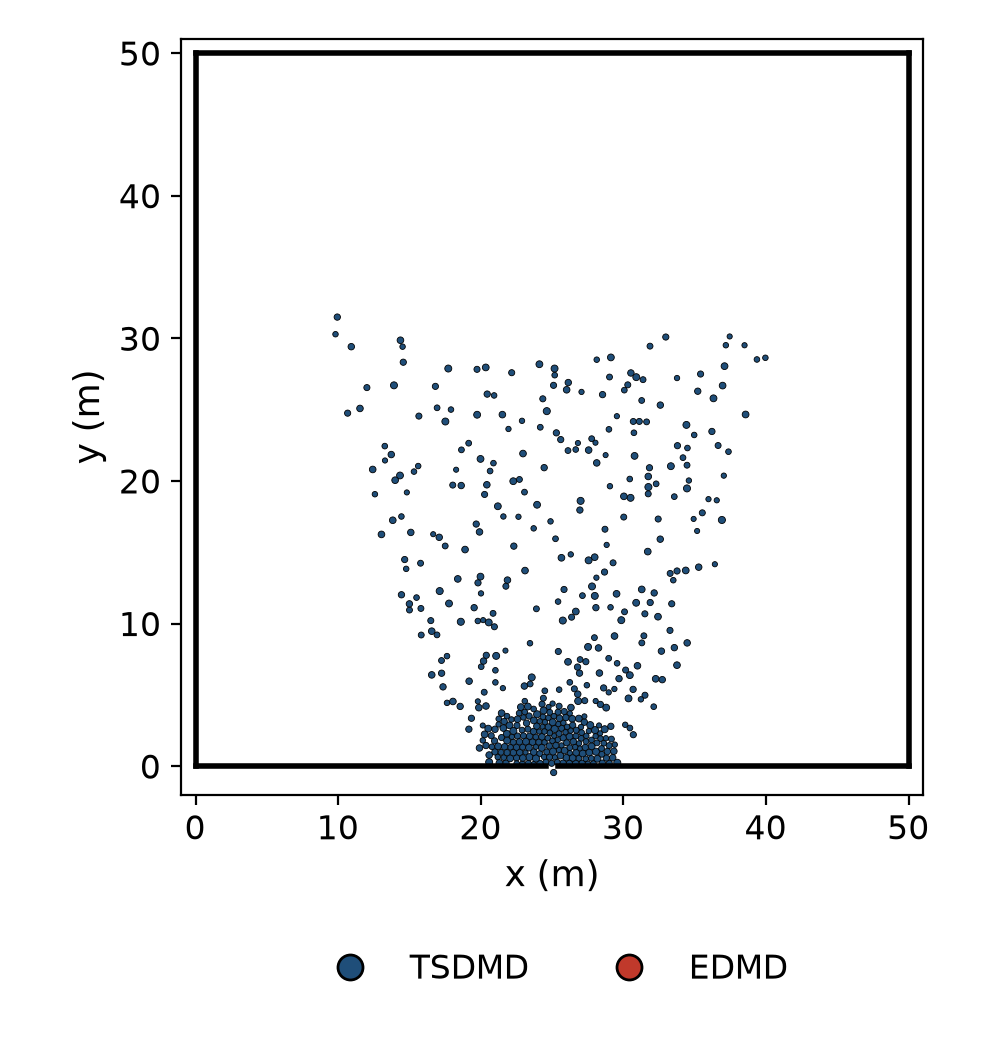
\includegraphics[width=0.74\linewidth]{frame_tsdmd.png}

      {\footnotesize\color{tsdmdc}\textbf{TSDMD}}\\
      \videolink{tsdmd_n500}
    \end{column}
    \begin{column}{0.325\textwidth}
      \centering
      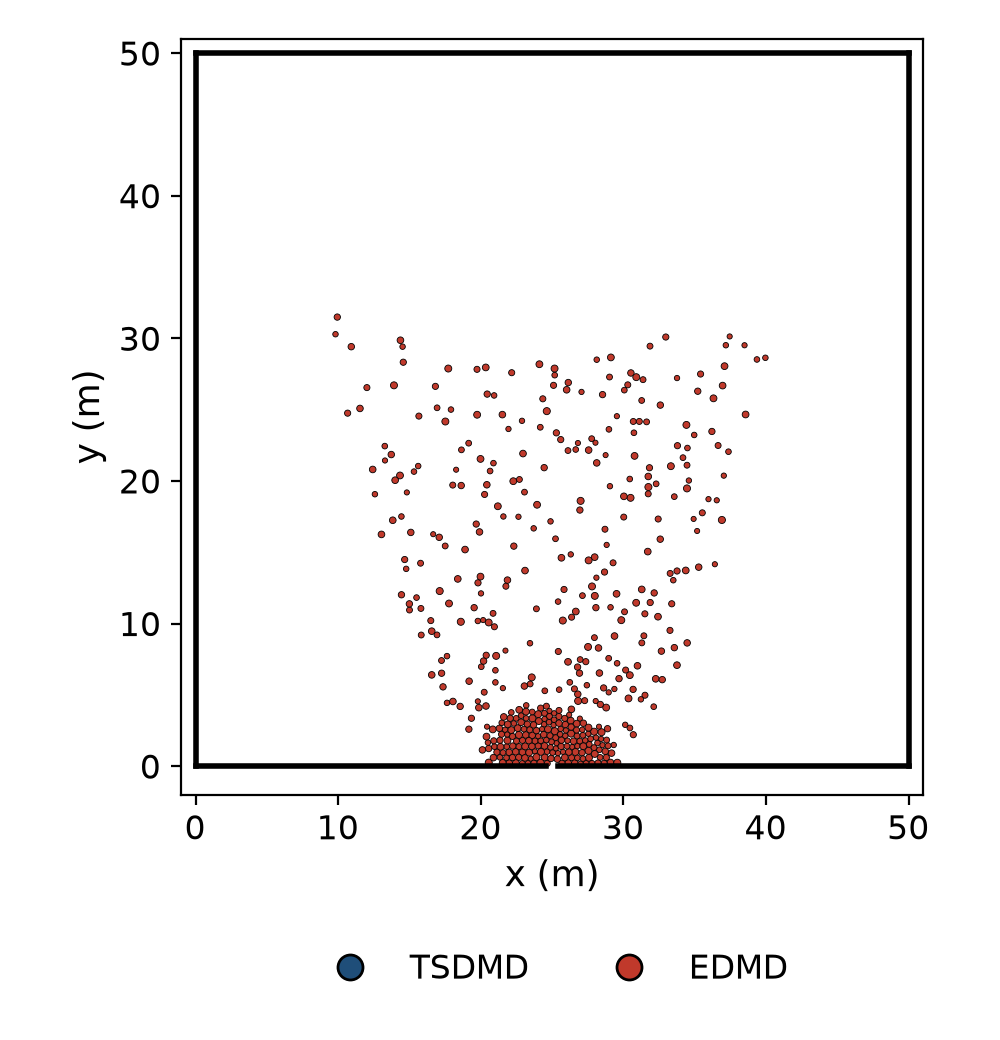
\includegraphics[width=0.74\linewidth]{frame_edmd.png}

      {\footnotesize\color{edmdc}\textbf{EDMD}}\\
      \videolink{edmd_n500}
    \end{column}
    \begin{column}{0.325\textwidth}
      \centering
      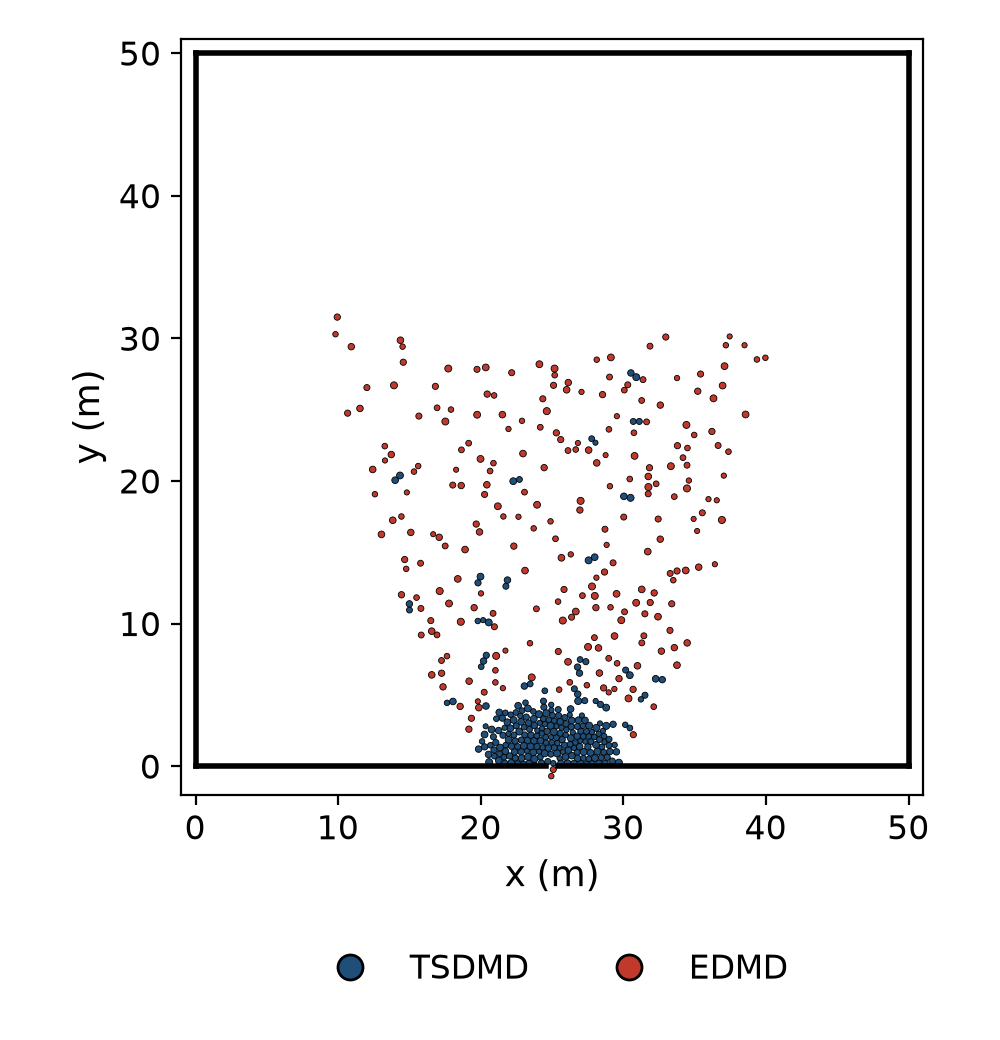
\includegraphics[width=0.74\linewidth]{frame_hybrid.png}

      {\footnotesize\color{hybc}\textbf{Híbrido}}\\
      \videolink{hybrid_n500}
    \end{column}
  \end{columns}
  \vfill
  \params{$N = 500$, $L = 50\un{m}$, semilla 18, $t = \framet\un{s}$; híbrido con $T = 0.5\un{s}$,
  $\alpha = 2$. Azul: TSDMD; rojo: EDMD (el híbrido colorea cada agente por su esquema vigente).}
\end{frame}

% SLIDE res_fraccion | V:C | T:30
\begin{frame}{Fracción de agentes por esquema en el híbrido}
  \begin{columns}[c]
    \begin{column}{0.64\textwidth}
      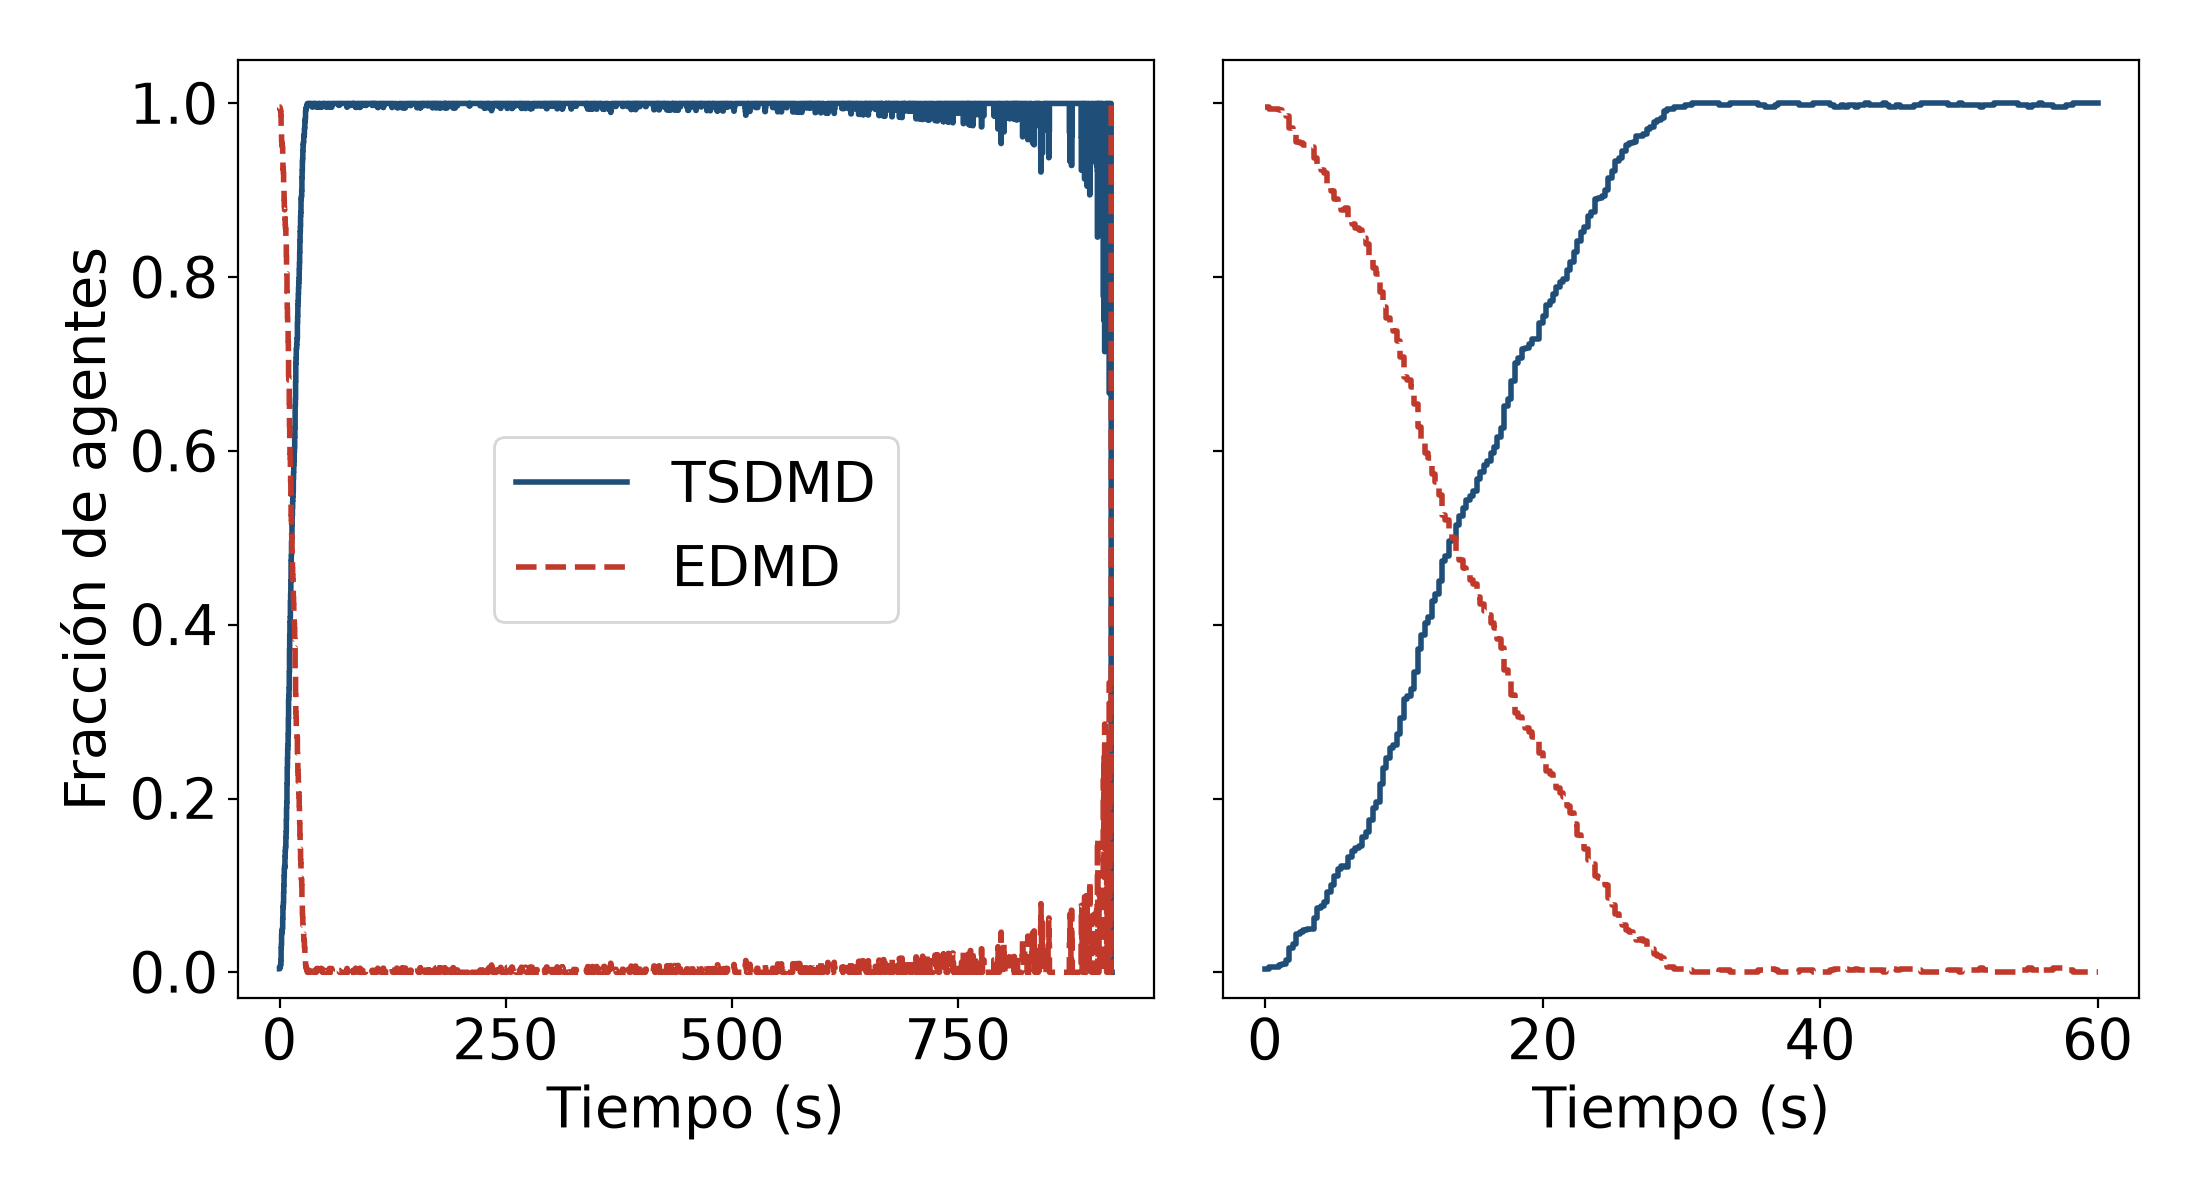
\includegraphics[width=\linewidth,height=0.84\textheight,keepaspectratio]{pres_fraction.png}
    \end{column}
    \begin{column}{0.34\textwidth}
      \params{%
        $N = 500$, $L = 50\un{m}$\\
        $T = 0.5\un{s}$, $\alpha = 2$\\
        semilla 18}

      \vspace{6pt}
      {\small Al inicio los agentes dispersos están en EDMD; hacia los $30\un{s}$ casi todos
      pasan a TSDMD (cuello de botella). Fracción TSDMD media de la corrida: $0.98$.}
    \end{column}
  \end{columns}
\end{frame}

% SLIDE res_poblacion | V:C | T:30
\begin{frame}{Población en la sala en función del tiempo}
  \begin{columns}[c]
    \begin{column}{0.64\textwidth}
      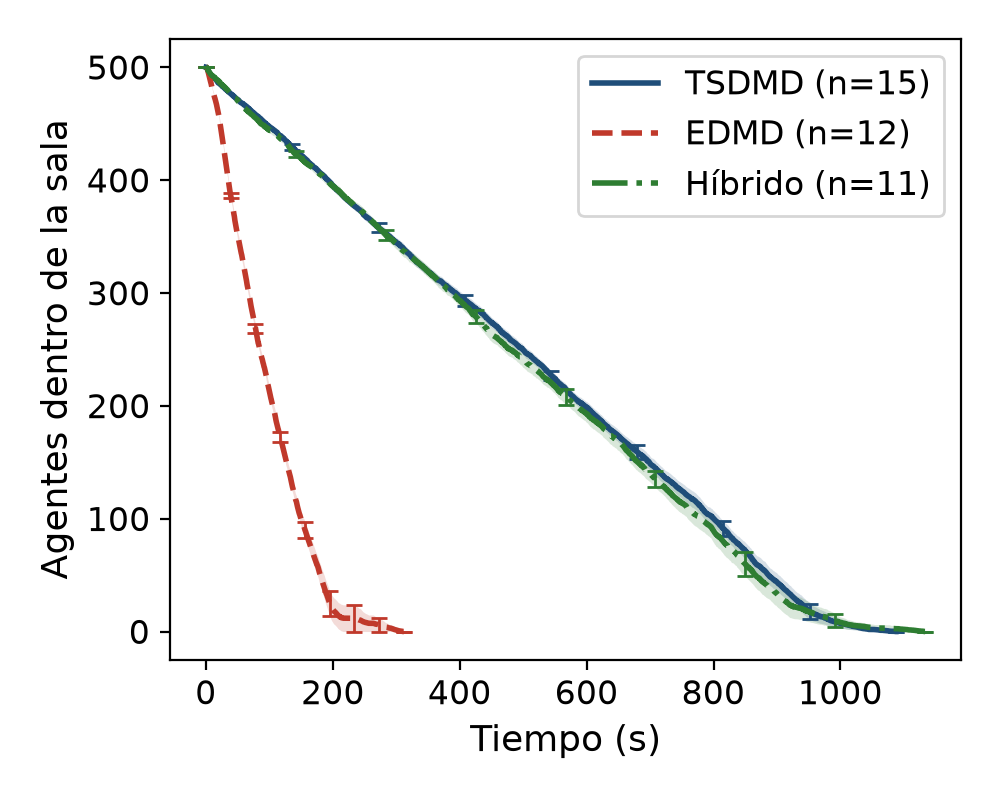
\includegraphics[width=\linewidth,height=0.84\textheight,keepaspectratio]{pres_population.png}
    \end{column}
    \begin{column}{0.34\textwidth}
      \params{%
        $N = 500$, $L = 50\un{m}$\\
        $T = 0.5\un{s}$, $\alpha = 2$\\[4pt]
        Solo corridas completas:\\
        TSDMD $n = 15$\\
        EDMD $n = 12$\\
        Híbrido $n = 11$}

      \vspace{6pt}
      {\small Las curvas del TSDMD y del híbrido casi se superponen; la del EDMD llega a $0$
      hacia los $300\un{s}$.}
    \end{column}
  \end{columns}
\end{frame}

% SLIDE res_tevac | V:C | T:40
\begin{frame}{Tiempo de evacuación según el esquema}
  \begin{columns}[c]
    \begin{column}{0.40\textwidth}
      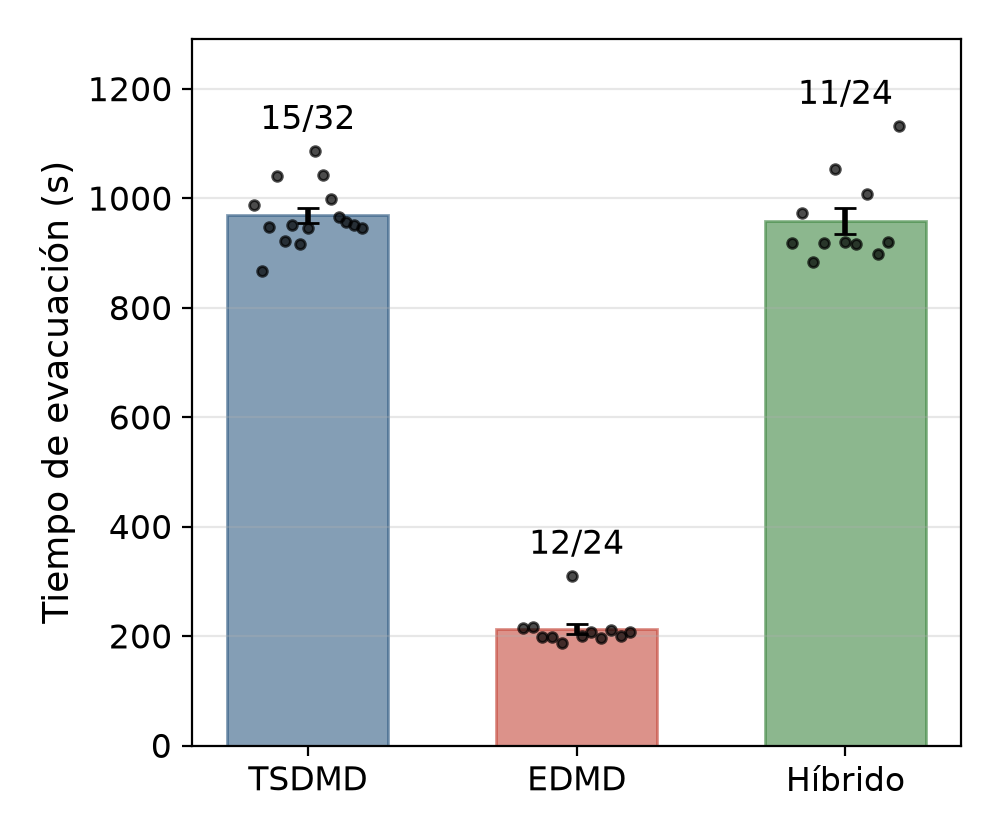
\includegraphics[width=\linewidth,height=0.84\textheight,keepaspectratio]{pres_tevac.png}
    \end{column}
    \begin{column}{0.58\textwidth}
      \resizebox{\linewidth}{!}{\tablaTevac}

      \vspace{4pt}
      \params{$N = 500$, $L = 50\un{m}$, $T = 0.5\un{s}$, $\alpha = 2$;
      $t_{max}$ 3000, 600 y $3000\un{s}$. Promedios solo sobre corridas completas.}

      \vspace{4pt}
      {\small EDMD: razón $0.22$ contra el TSDMD, $z = -44$. Híbrido: razón $0.99$ y
      $z = -0.4$, no distinguible del TSDMD con $n = 11$ y $15$.}
    \end{column}
  \end{columns}
\end{frame}

% SLIDE res_walltime | V:C | T:30
\begin{frame}{Tiempo de ejecución según el esquema}
  \begin{columns}[c]
    \begin{column}{0.40\textwidth}
      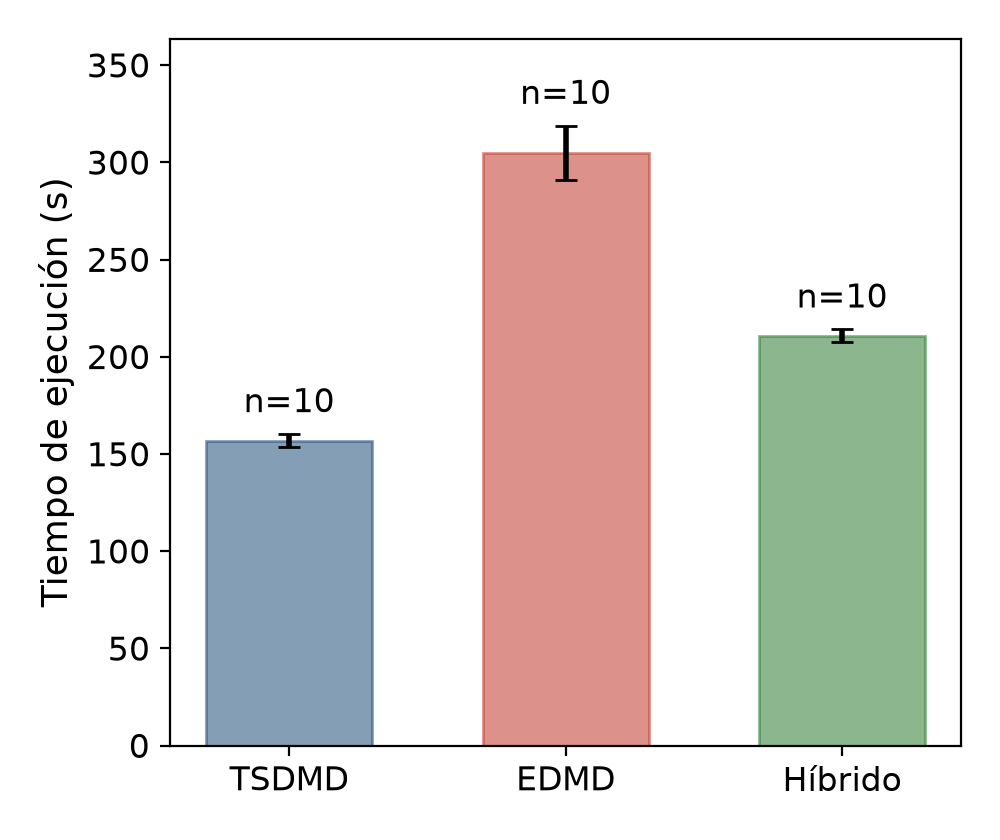
\includegraphics[width=\linewidth,height=0.84\textheight,keepaspectratio]{pres_walltime.png}
    \end{column}
    \begin{column}{0.58\textwidth}
      \resizebox{\linewidth}{!}{\tablaWall}

      \vspace{4pt}
      \params{$N = 500$, $L = 50\un{m}$, un hilo; 10 corridas completas por esquema.}

      \vspace{4pt}
      {\small Orden de costo: TSDMD, híbrido ($\times1.34$) y EDMD ($\times1.94$), inverso
      al orden de $t_{evac}$.}
    \end{column}
  \end{columns}
\end{frame}

% SLIDE res_sweep | V:C | T:40
\begin{frame}{Barrido de $T$ en el híbrido}
  \begin{columns}[c]
    \begin{column}{0.40\textwidth}
      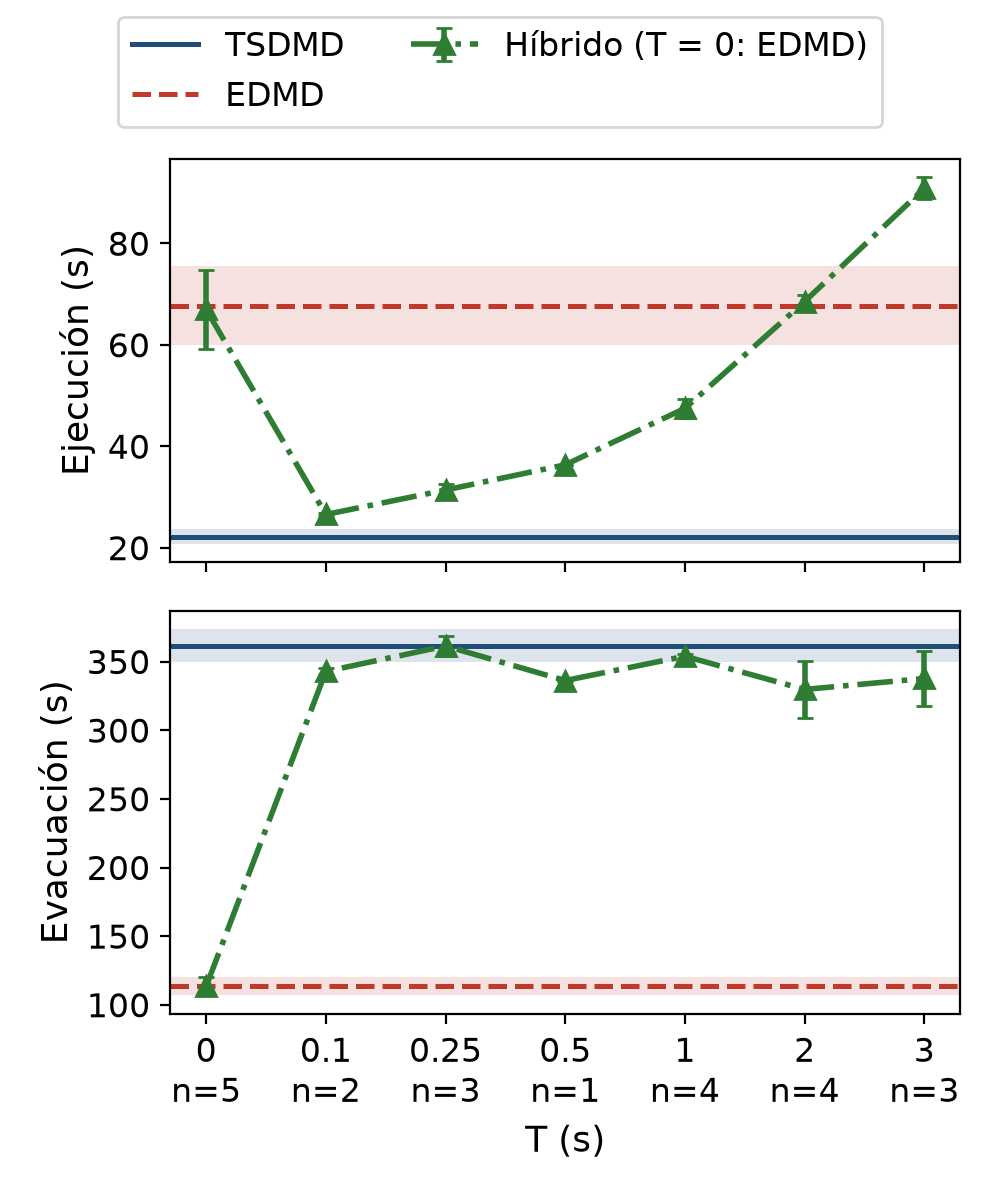
\includegraphics[width=\linewidth,height=0.84\textheight,keepaspectratio]{pres_sweep_T.png}
    \end{column}
    \begin{column}{0.58\textwidth}
      \params{$N = 200$, $L = 31.6\un{m}$, $\alpha = 2$, 5 semillas por $T$,
      $t_{max} = 600\un{s}$; $n$ completas por $T$ en el eje.}

      \vspace{6pt}
      \small
      \begin{itemize}
        \item $T = 0$ reproduce al EDMD (trayectorias idénticas).
        \item Para $T > 0$ el $t_{evac}$ queda del lado del TSDMD: ningún $T$ evaluable difiere
          en más de $2$ errores combinados; $T = 0.5\un{s}$ tiene una sola completa y no se evalúa.
        \item Tiempo de ejecución mínimo en $T = 0.1\un{s}$ ($n = 2$); crece con $T$.
      \end{itemize}
    \end{column}
  \end{columns}
\end{frame}

% SLIDE res_scale_a | V:C | T:30
\begin{frame}{Escalado en $N$: densidad inicial constante}
  \begin{columns}[c]
    \begin{column}{0.46\textwidth}
      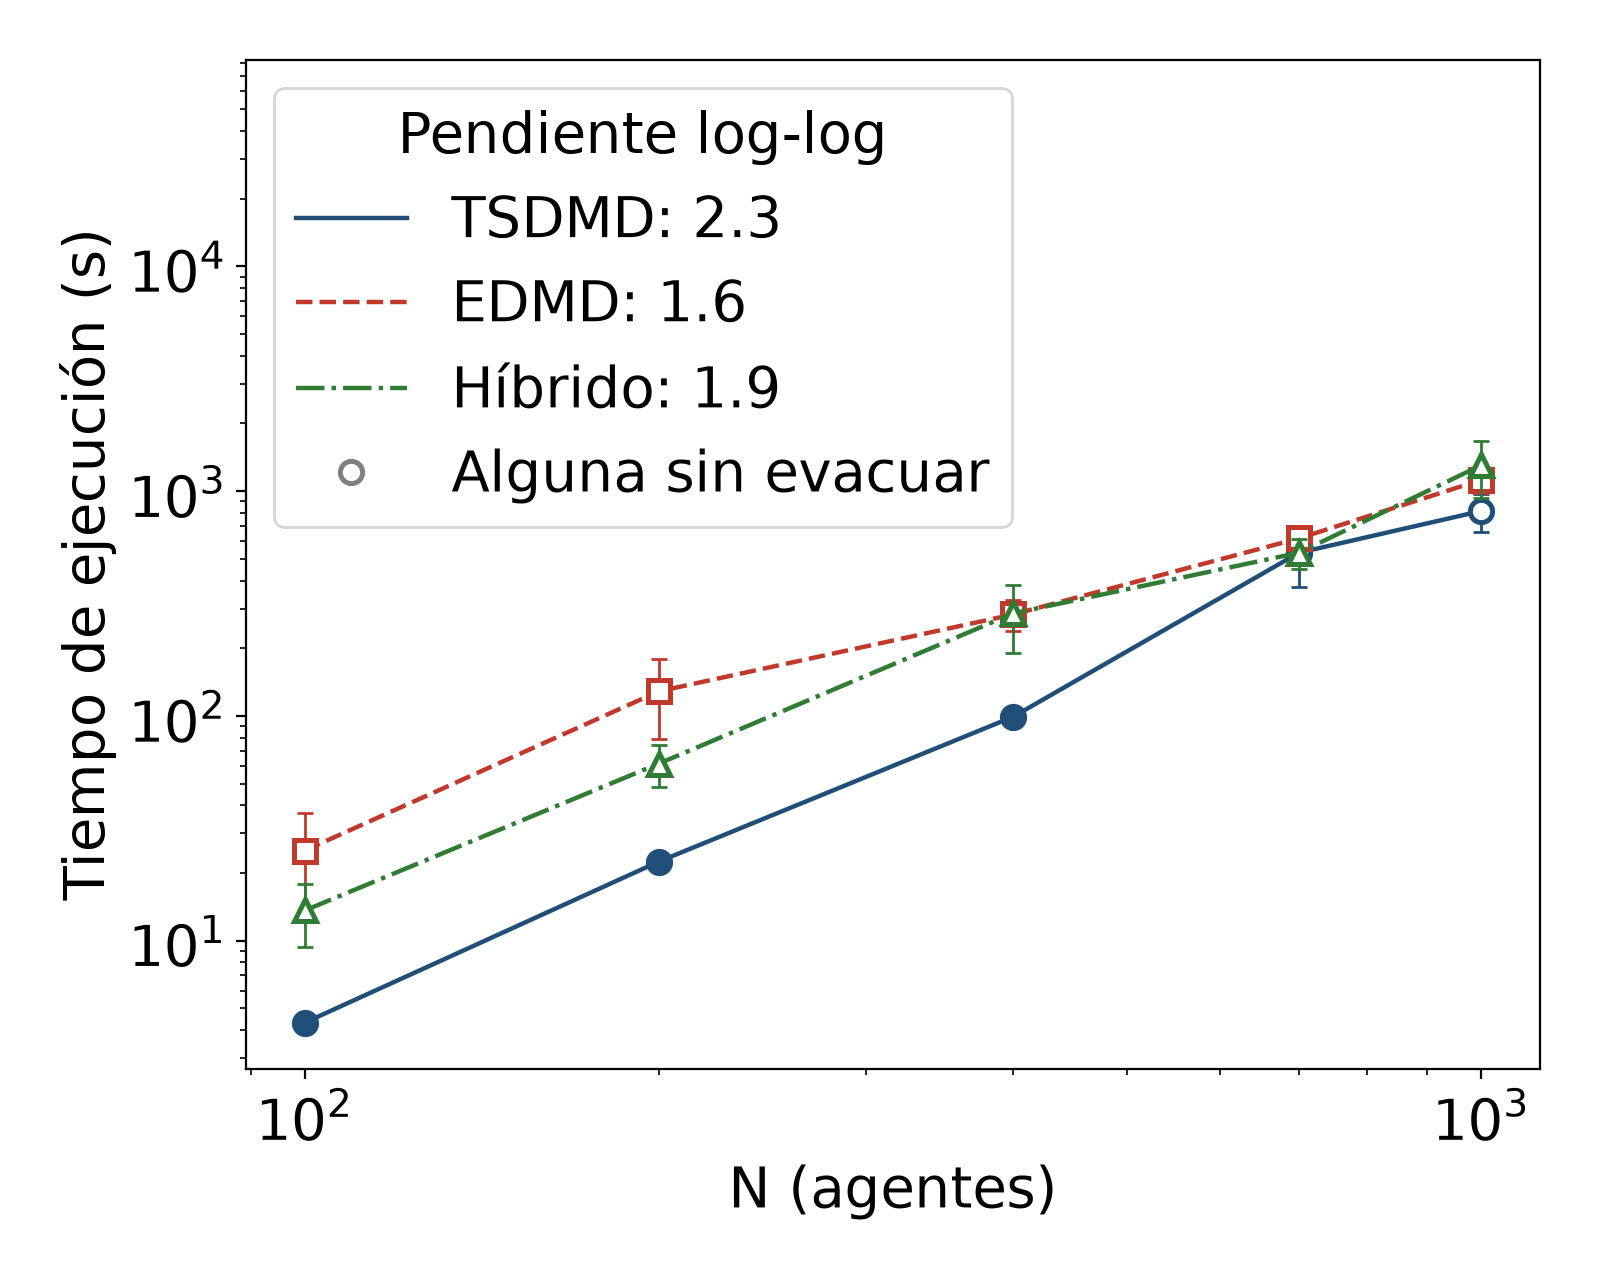
\includegraphics[width=\linewidth,height=0.84\textheight,keepaspectratio]{pres_scale_a.png}
    \end{column}
    \begin{column}{0.52\textwidth}
      \params{$N\in\{100,\,200,\,400,\,700,\,1000\}$, $L = 50\sqrt{N/500}\un{m}$,
      3 semillas por punto, $t_{max}\propto N$. Marcador hueco: alguna corrida llegó a $t_{max}$
      sin evacuar ($18$ de $45$).}

      \vspace{6pt}
      {\small Pendiente de la media observada: TSDMD $2.3$, EDMD $1.6$, híbrido $1.9$.
      \textbf{No son exponentes de costo.} Para $N\ge700$ los esquemas no se separan dentro
      del error con $3$ realizaciones por punto.}
    \end{column}
  \end{columns}
\end{frame}

% SLIDE res_scale_b | V:C | T:30
\begin{frame}{Escalado en $N$: sala fija}
  \begin{columns}[c]
    \begin{column}{0.46\textwidth}
      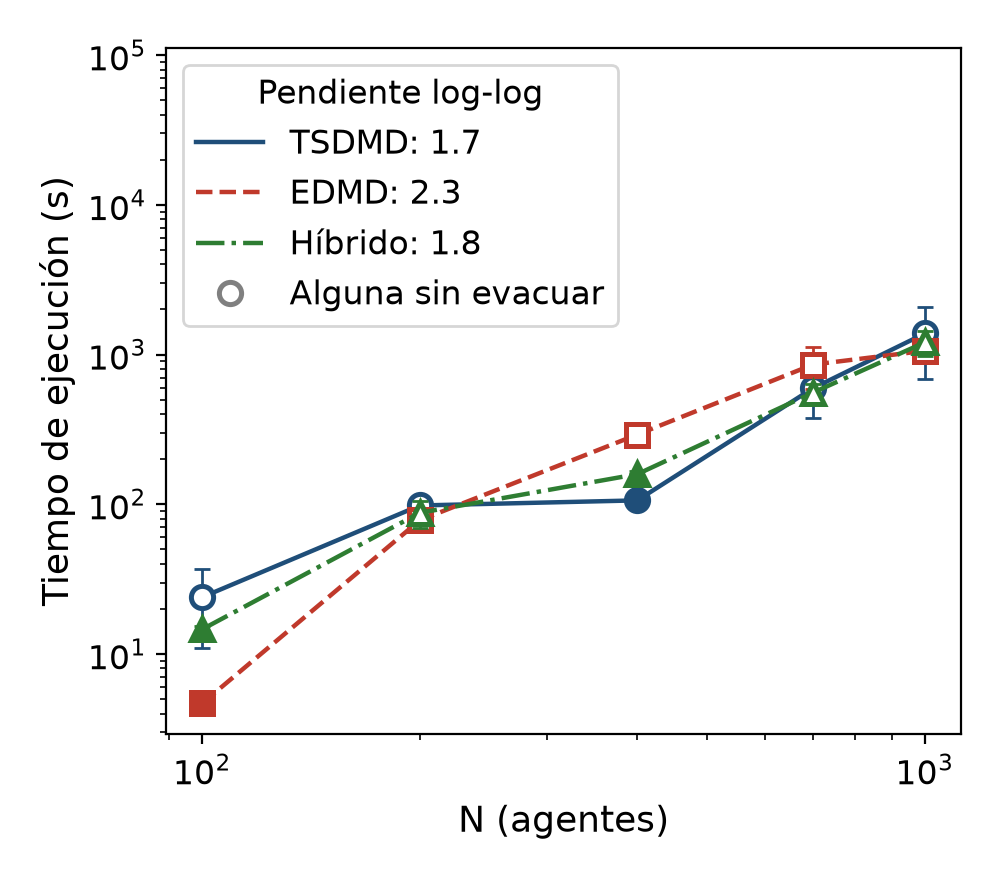
\includegraphics[width=\linewidth,height=0.84\textheight,keepaspectratio]{pres_scale_b.png}
    \end{column}
    \begin{column}{0.52\textwidth}
      \params{$N\in\{100,\,200,\,400,\,700,\,1000\}$, $L = 50\un{m}$,
      3 semillas por punto, $t_{max}\propto N$. Marcador hueco: alguna corrida llegó a $t_{max}$
      sin evacuar ($20$ de $45$).}

      \vspace{6pt}
      {\small Pendiente de la media observada: TSDMD $1.7$, EDMD $2.3$, híbrido $1.8$.
      \textbf{No son exponentes de costo.} Para $N\ge700$ los esquemas no se separan dentro
      del error con $3$ realizaciones por punto.}
    \end{column}
  \end{columns}
\end{frame}


% =====================================================================
\section{Conclusiones}
% =====================================================================
%  Conclusiones (una diapositiva, solo lo mostrado en resultados; Guia 2.5) y cierre
% =====================================================================

% SLIDE concl | V:A | T:40
\begin{frame}{Conclusiones}
  \small
  \begin{enumerate}
    \item El EDMD evacua la sala mucho más rápido que el TSDMD; el híbrido no se distingue del
      TSDMD en el tiempo de evacuación, y ningún $T > 0$ evaluable lo cambia. Con $T$ nulo se reproduce
      el EDMD.
    \item El costo de ejecución ordena TSDMD $<$ híbrido $<$ EDMD, inverso al del tiempo de
      evacuación: el híbrido no mejora al TSDMD con los criterios probados.
    \item El híbrido se parece al TSDMD porque casi todos los agentes están en TSDMD: la cola de
      la puerta es de contactos continuos.
    \item El híbrido no tiene colisiones duras; la auditoría no encontró contactos perdidos ni
      solapes de residentes EDMD.
    \item Para $N$ grande el escalado no separa los esquemas dentro del error.
  \end{enumerate}
\end{frame}

% SLIDE gracias | V:A | T:3
\begin{frame}
  \vfill
  \centering
  {\Large Muchas gracias}
  \vfill
\end{frame}


% =====================================================================
%  Apendice: uso de IA y libertades corregidas (T:0, fuera del presupuesto de tiempo)
% =====================================================================
\appendix

% SLIDE anexo_ia | V:A | T:0
\begin{frame}{Apéndice: uso de IA}
  \small
  \begin{itemize}
    \item Herramienta: Claude Code (agente de IA), con planes por fase y un resumen por plan.
    \item El agente escribió el motor C\texttt{++}20 (TSDMD, EDMD, híbrido), los \emph{scripts} de
      Python, las figuras, las animaciones y esta presentación.
    \item Supervisamos cada plan y corregimos lo que se tomó por su cuenta. Las siguientes
      diapositivas listan esas libertades, agrupadas por tipo.
    \item Cada punto sale de los desvíos registrados en los resúmenes de plan (\emph{Deviations}).
  \end{itemize}
\end{frame}

% SLIDE anexo_motor | V:A | T:0
\begin{frame}{Libertades en el motor que hubo que corregir}
  \footnotesize
  \begin{enumerate}
    \item \textbf{EDMD, piso de tiempo por agente:} para evitar el colapso inelástico puso un
      piso por agente; un agente atrapado dejaba contactos sin atender y llegó a solapes de
      0.49 m. Se pasó a un piso por contacto (par, pared o esquina).
    \item \textbf{EDMD, solapes en cadena:} proyectar todos los solapes (\texttt{--overlap-cap 0})
      daba 15 de 15 arcos estables a $N = 500$. Sin relajar el umbral de 0.09 m, elegimos un
      tope (\texttt{--overlap-cap} 0.07 m) entre las opciones que propuso.
    \item \textbf{Híbrido, \emph{ping-pong} entre esquemas:} decidía los retornos todos juntos;
      663 promociones y 661 retornos en $N = 8$. Se pasó a un retorno por vez.
    \item \textbf{Híbrido, oscilación en el límite entre esquemas:} el retorno modelaba al vecino
      a velocidad constante y el aviso a relajación a $v_d$; 61 de 122 retornos eran
      repromociones rápidas. Se exigió el contacto lejano bajo los dos modelos.
    \item \textbf{Contactos en reposo:} contaba como inaplicable un contacto con $v_n = 0$ por
      redondeo de $10^{-17}$ (112 de 1.5M eventos).
  \end{enumerate}
\end{frame}

% SLIDE anexo_atajos | V:A | T:0
\begin{frame}{Libertades al validar y al elegir corridas}
  \footnotesize
  \begin{enumerate}
    \item \textbf{Tolerancia de la prueba:} subió la tolerancia del comparador de la cola de
      eventos de $10^{-7}$ a $10^{-5}$ s. Pedimos controles negativos que demuestren que sigue
      detectando eventos perdidos y espurios.
    \item \textbf{Semillas que completan:} para humos, determinismo y referencias fue eligiendo
      semillas que evacúan (3, 5, 10, 17) y descartando arcos. Lo corregimos reportando siempre
      la tasa de éxito y promediando solo corridas completas ($\geq 10$ por esquema).
    \item \textbf{Escenarios de prueba a medida:} cambió a mano $\alpha$, posiciones iniciales y
      el sesgo de los casos aleatorios para que la prueba ejercite lo pedido; revisamos que
      ningún ajuste cambie el motor ni los umbrales.
    \item \textbf{Requisitos cerrados antes de tiempo:} marcó STUDY-04 a STUDY-07 como completos
      cuando solo existían las herramientas, sin datos. Se reabrieron hasta tener las corridas.
    \item \textbf{Mecanismos sin medir:} explicaba el costo con hipótesis. Se exigió citar solo
      contadores medidos (\texttt{study\_counters.py}) y marcar el resto como hipótesis.
  \end{enumerate}
\end{frame}

% SLIDE anexo_proceso | V:A | T:0
\begin{frame}{Libertades de proceso, herramientas y formato}
  \footnotesize
  \begin{enumerate}
    \item \textbf{\texttt{git commit}:} el coordinador pidió commits atómicos por tarea contra
      nuestra regla de que commiteamos nosotros; se cumplió la regla y no se commiteó.
    \item \textbf{Orden de trabajo:} en varios planes escribió la implementación antes que las
      pruebas, aunque el plan pedía lo contrario.
    \item \textbf{Alcance:} agregó clases, funciones y archivos no pedidos (p.\,ej.
      \texttt{FfmpegUnavailable}, \texttt{spec\_from\_row}, \texttt{frame\_t.tex}) y un programa
      auxiliar de calibración fuera del proyecto.
    \item \textbf{Falsos fallos de verificación:} comparar el \texttt{sha256} del zip daba FAIL
      entre Windows y WSL (versión de zlib); \texttt{python3 -I} no veía \texttt{matplotlib}; un
      patrón de ruta local confundió una fórmula en LaTeX.
    \item \textbf{Formato:} \texttt{babel-spanish} puso coma decimal en modo matemático; la
      anotación \emph{completas/intentadas} de una figura tapaba los puntos; texto de figuras de
      6 a 7 pt. Se corrigieron al revisar la salida.
  \end{enumerate}
\end{frame}

\end{document}
